\documentclass[11pt]{article}
\usepackage[margin=1.05in]{geometry}
\usepackage{amsmath,amssymb}
\usepackage{graphicx}
\usepackage{booktabs}
\usepackage{xcolor}
\usepackage[colorlinks=true,linkcolor=blue!55!black,urlcolor=blue!55!black]{hyperref}
\usepackage{microtype}

\title{Walkthrough: the Slosh Mechanism and the Parity Measurement\\
\large Q2.1 of the PI-question analyses, slowly, piece by piece\\
(companion to \texttt{pi\_questions\_analysis.ipynb}, \S Q2.1)}
\author{}
\date{2026-08-20}

\newcommand{\dd}{\mathrm{d}}
\begin{document}
\maketitle

\noindent Setting: the $4\pi G = 6$, amp $= 0.2$ swing-collapse runs. The question
being explained: how the collapse chooses its site, and how we established that the
mirror symmetry of the problem is preserved by the code. Every claim below points at
a measured curve in the figures.

%=====================================================================
\section{The slosh mechanism: how the collapse chooses its site}

\subsection*{Step 1 --- what ``the site'' means}
After fragmentation, one dominant knot forms on the corotation column $x \approx 0$.
The mirror symmetry (\S2) allows exactly two single-knot sites there: $y = 0$
(``center'') and $y = \pm\pi$ (``wrap''). The puzzle: from identical initial
conditions, the $128^2$ run picked center and the $256^2$ runs picked the wrap.
Which site wins, and why does it depend on resolution?

\subsection*{Step 2 --- the collapse is not one-shot}
Follow the gray max-density curve in Fig.~\ref{fig:slosh}. The swing compresses the
crest to $\rho \approx 10$--20 around $t \approx 4.5$--5 --- and then the crest
\emph{bounces}: pressure wins, and by $t = 6$--8 the maximum is back down to
$\rho \approx 2$. The famous ``fragmentation at $t \approx 4.5$'' is the beginning
of a long negotiation, not the final collapse. The real runaway happens three to
five time units later, out of the bounced debris.

\subsection*{Step 3 --- what oscillates in the interlude}
Take the corotation column's density profile $\rho(y)$ and project it onto
$\cos y$ and $\sin y$ (the $m{=}1$ Fourier coefficient $c_1$). Its magnitude
$|c_1|$ says how much density contrast the column carries; its phase says
\emph{where} the pile-up is. Because of the mirror symmetry the phase can only be
$0$ or $\pi$ (\S2, Step~6): the pattern is a \textbf{standing wave} that alternately
piles density at $y = 0$ (blue points in Fig.~\ref{fig:slosh}) and at $y = \pm\pi$
(orange points), passing through zero contrast at each flip.

\subsection*{Step 4 --- why it oscillates instead of growing}
By $t \approx 7$ the wave has rewound to $k_x = -6 + 1.5t \approx 4.5$, so
$k = \sqrt{k_x^2 + k_y^2} \approx 4.6$, and the local dispersion relation gives
\begin{equation}
\omega^2 = \kappa^2 + c_s^2 k^2 - 4\pi G \rho_0 \;\approx\; 1 + 21 - 6 = +16 > 0 :
\end{equation}
pressure has re-stabilized the winding wave --- it \emph{rings} instead of growing,
with period $2\pi/\omega \approx 1.6$, i.e.\ a site flip every $\approx 0.8$. That
matches the measured flip cadence in Fig.~\ref{fig:slosh}; and since $k(t)$ keeps
growing, the flips accelerate toward $t = 9$--10, exactly as the $256^2$ panel
shows. (This is the same physics as the movie-flicker ringing of Q0.2, now with
self-gravity in the frequency.)

\subsection*{Step 5 --- the trigger}
Meanwhile the bounced debris slowly re-contracts: the gray curve creeps from
$\rho \approx 2$ up through $\approx 10$ over $t = 7$--9. A knot goes into runaway
when its \emph{local} Jeans length $\lambda_J \propto \rho^{-1/2}$ drops below its
own size --- after that, the gray curve goes vertical. Measured onset (last upward
crossing of $\rho = 20$): $t = 8.80$ at $128^2$, $t = 9.45$ at $256^2$.

\subsection*{Step 6 --- the selection}
The runaway grabs the densest material \emph{at the moment it fires} --- and where
that is alternates with the slosh. At $128^2$ the onset lands on a $y{=}0$ phase
(blue, $|c_1|$ risen to $1.5$): clump at center, $(+0.025, -0.025)$. At $256^2$ the
onset comes half a slosh cycle later and settles on a $\pi$ phase: knot at the
wrap. Same mechanism, opposite outcomes, decided by a $\approx 0.65$ timing offset.

\subsection*{Step 7 --- why the resolutions fire at different times}
Through the swing the two runs are essentially identical ($d_{\cos}$ agrees to 2--3
digits at $t \le 5$). The \emph{bounce}, however, compresses the crest to near the
grid scale at $128^2$ --- this run exceeds its Truelove ceiling, the documented
marginality --- and that is precisely where resolution matters. The post-bounce
trajectories drift apart, the $128^2$ run tips over earlier, and the half-cycle
offset flips the site. Not randomness: a deterministic, symmetric double-well
decision balanced on a knife edge. The converged answer is the wrap: MG $256^2$,
FFT $256^2$, and the AMR run (fine level $\equiv 256^2$) all agree.

\begin{figure}[htb]
\centering
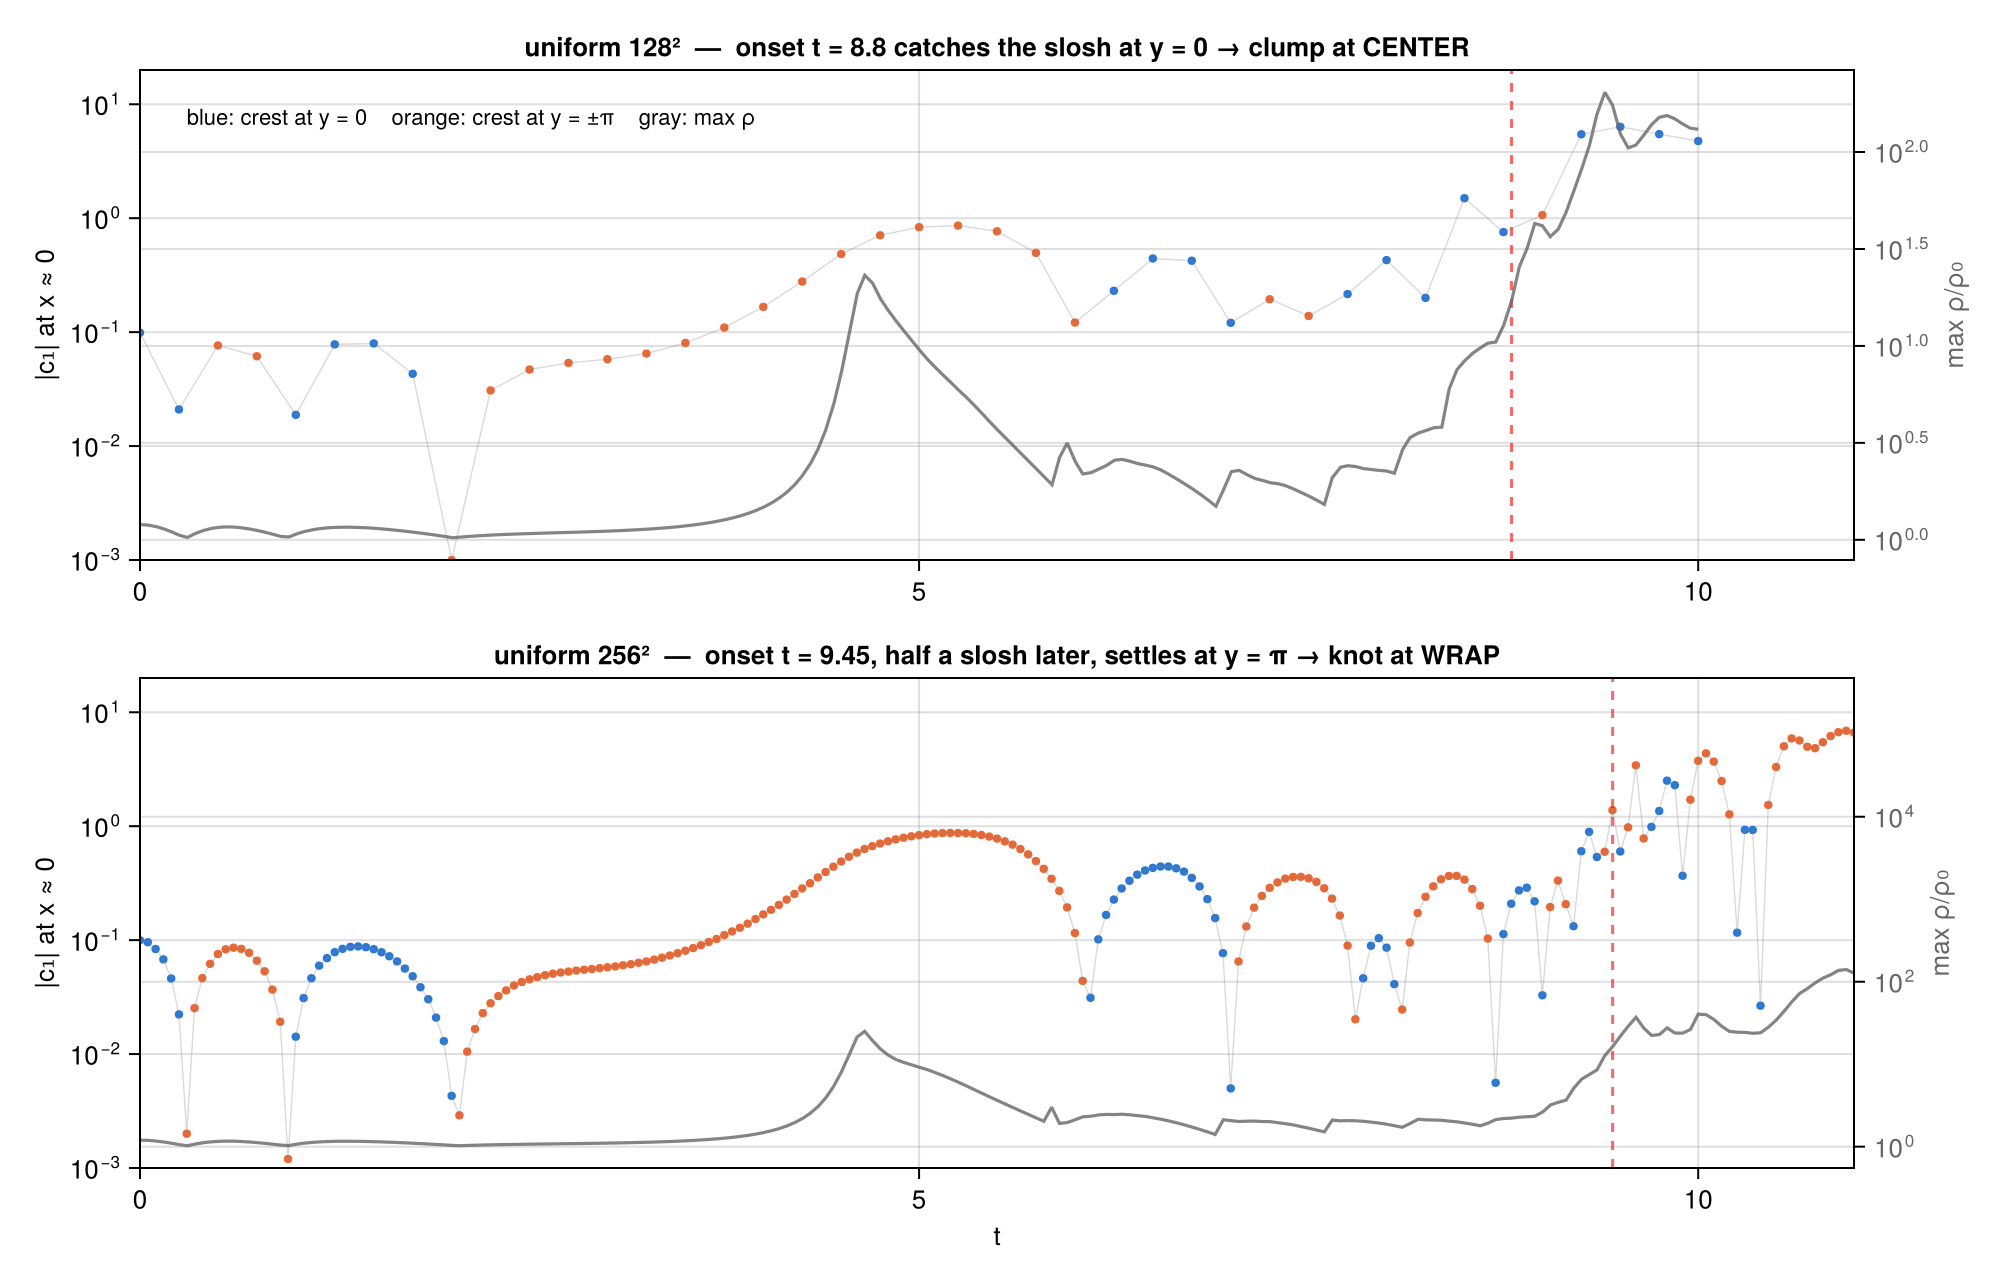
\includegraphics[width=\textwidth]{figures/pi_q21_slosh.png}
\caption{The slosh and the onset. Points: corotation-column $m{=}1$ amplitude
$|c_1|$, colored by which site holds the density (blue $y{=}0$, orange
$y{=}\pm\pi$); gray: max density; red dashed: runaway onset ($\rho$ crosses 20).}
\label{fig:slosh}
\end{figure}

\begin{figure}[htb]
\centering
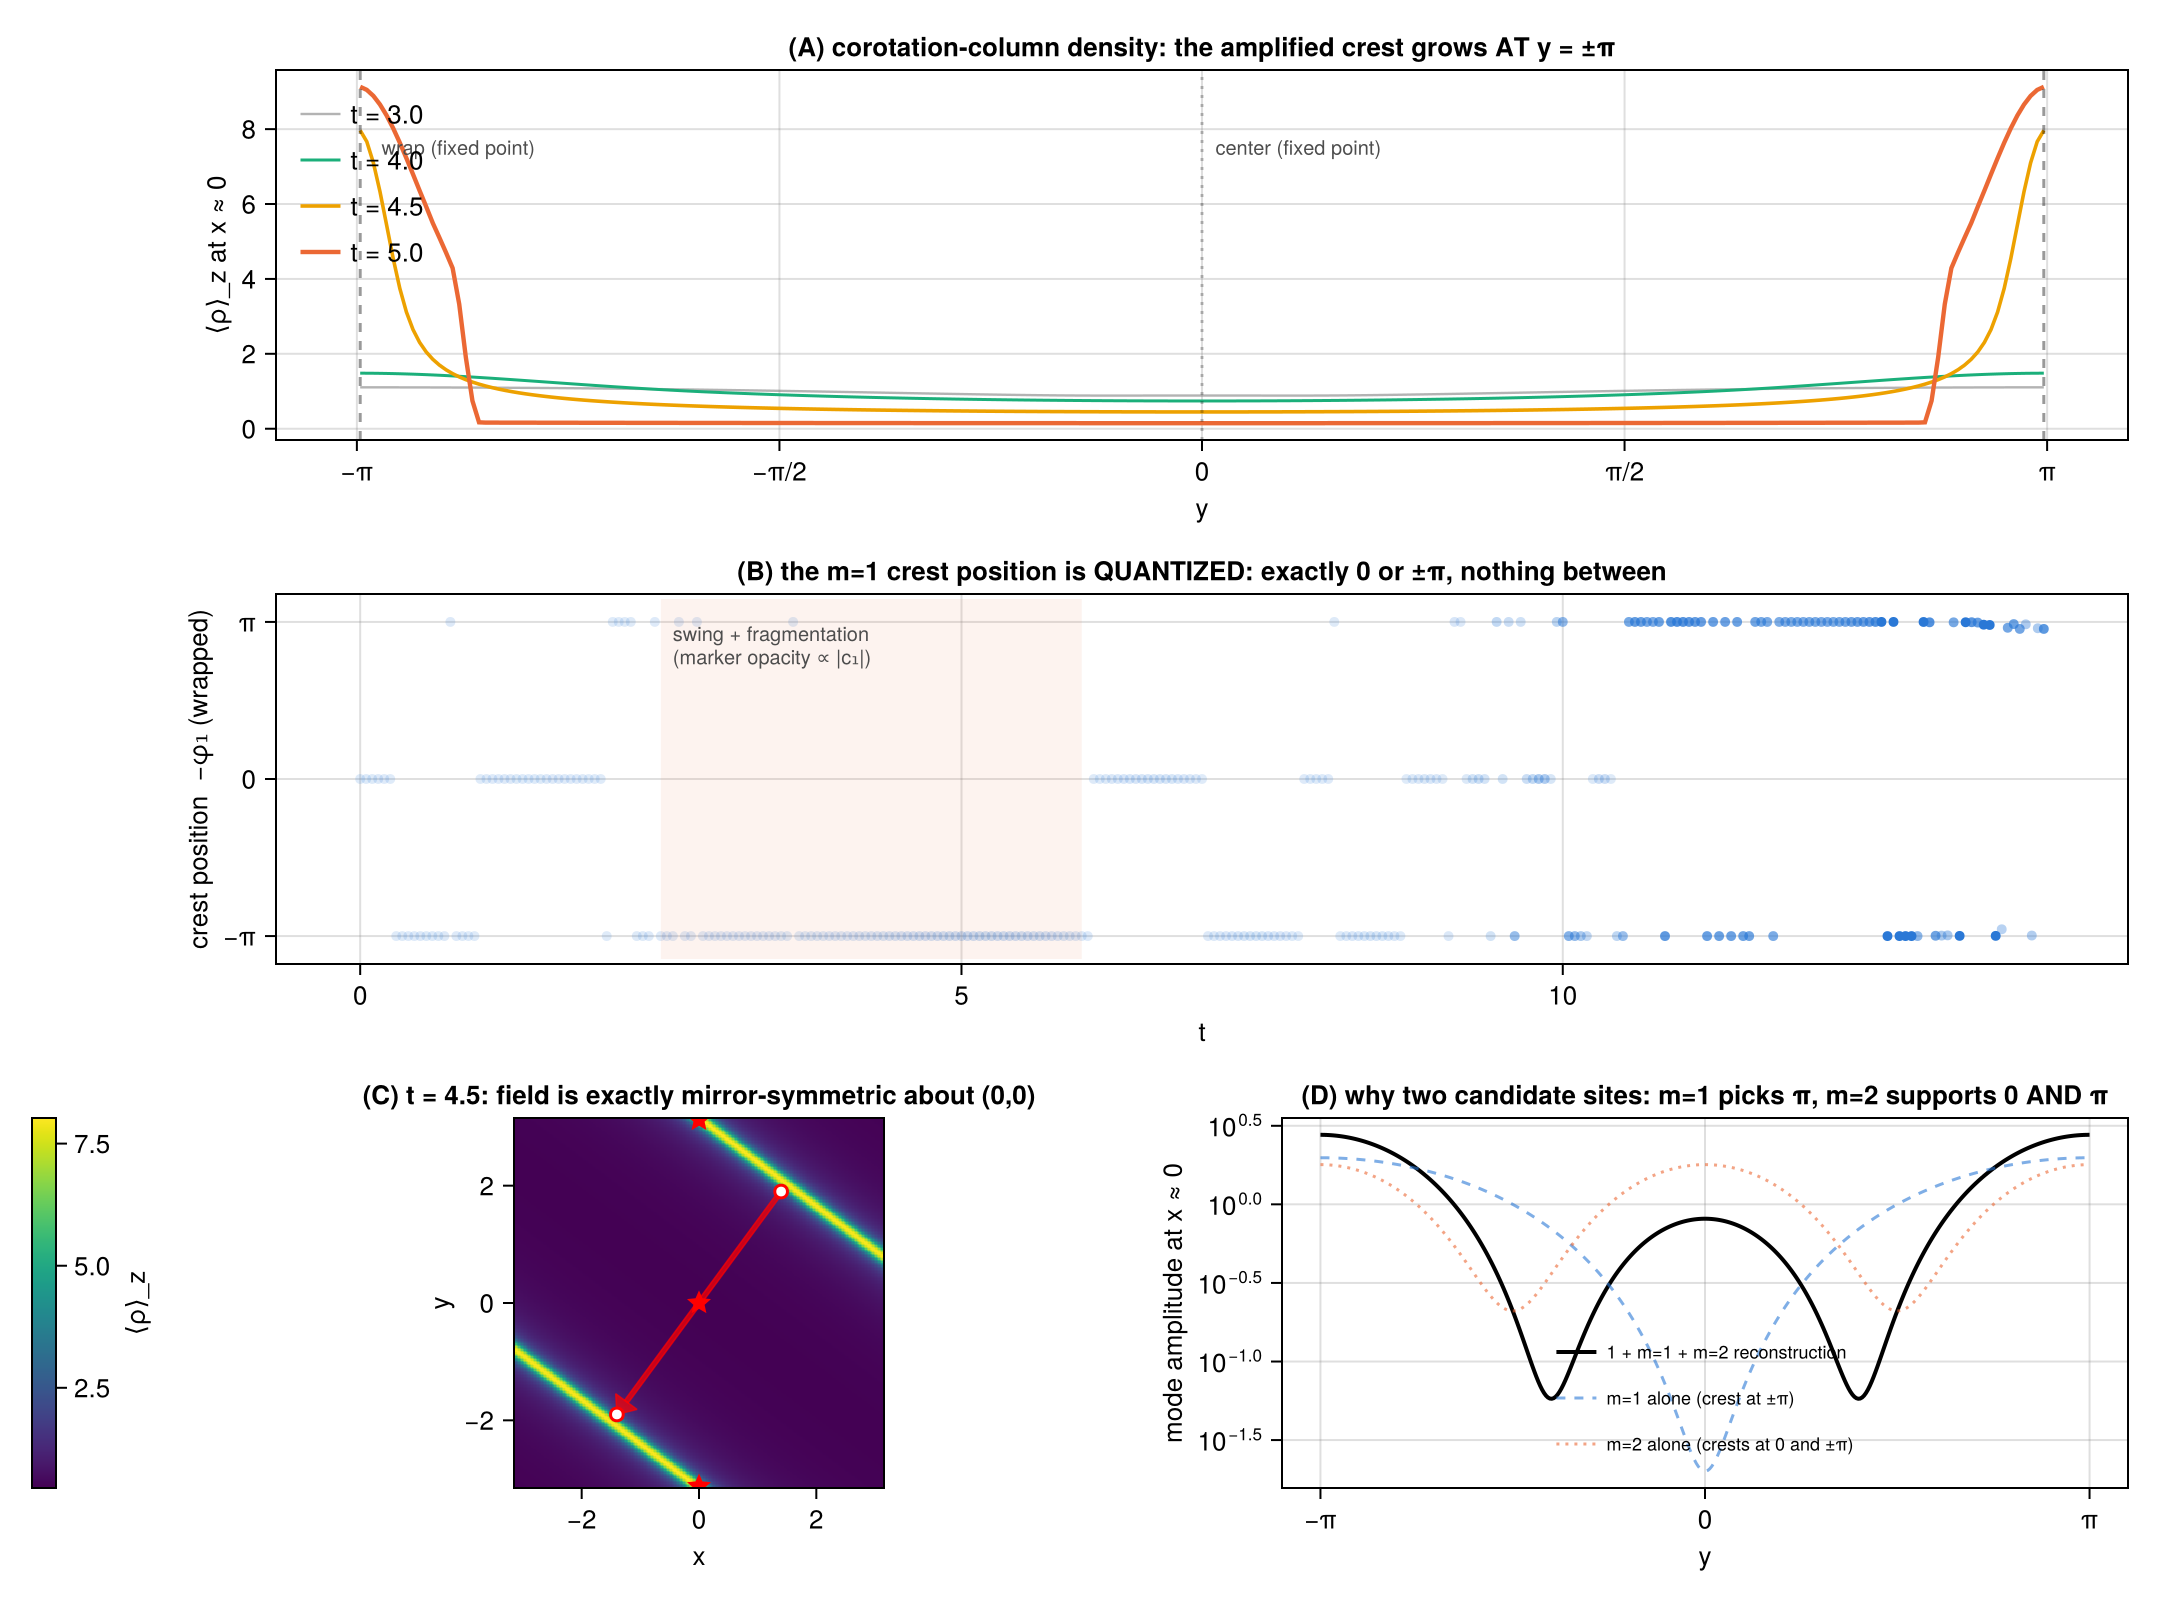
\includegraphics[width=\textwidth]{figures/pi_q21_quantization.png}
\caption{Why only two sites exist. (A) corotation-column profiles: the amplified
crest grows at $y = \pm\pi$; (B) the measured crest position takes only the values
$0$ and $\pm\pi$; (C) the $t{=}4.5$ field with its mirror-symmetric structure
(stars: fixed points; white dots: a mirror pair); (D) the $m{=}1 + m{=}2$
reconstruction of the column showing the two candidate sites.}
\label{fig:quant}
\end{figure}

\clearpage
%=====================================================================
\section{The parity measurement}

\subsection*{Step 1 --- the symmetry being tested}
The point reflection $P:(x,y) \to (-x,-y)$. The initial condition has it because
cosine is even: $\cos(-k\!\cdot\!x) = \cos(k\!\cdot\!x)$. The \emph{dynamics} keeps
it because every term of the shearing-box equations transforms consistently under
$P$ (with velocities flipping sign): the background shear $-q\Omega x$ is odd in
$x$, and Coriolis, tidal, pressure, and self-gravity terms all commute with the
reflection. Crucially this holds at \emph{any} amplitude --- symmetry is not a
linear-theory statement. So a $P$-even density field must stay $P$-even forever;
any deviation is numerical.

\subsection*{Step 2 --- the metric}
Compare the field with its own reflection, snapshot by snapshot:
\begin{equation}
a(t) \;=\; \max_{i,j}\;\big|\,S(i,j) - S(\text{mirror}(i,j))\,\big|
\end{equation}
on the $z$-averaged density $S$. $a = 0$ means the two mirror halves of the stored
field are \textbf{bitwise identical} --- all 32{,}768 mirror pairs, to the last bit.

\subsection*{Step 3 --- the grid subtlety}
Cell centers sit at $\pm\Delta/2, \pm3\Delta/2,\ldots$; no cell lies at the origin.
The mirror of cell index $i$ is therefore $\mathrm{mod1}(257 - i,\,256)$, pairing
$+\Delta/2$ with $-\Delta/2$. An off-by-one here (mirror $= 258 - i$) misaligns
every pair by one cell and reports a large \emph{false} asymmetry --- I made
exactly that mistake on the first attempt. The self-check that catches it: the
$t = 0$ initial condition must give $a = 0$ exactly.

\subsection*{Step 4 --- reading the curve (Fig.~\ref{fig:parity})}
Three regimes:
\begin{enumerate}
\item \textbf{The exact-zero rail}, through $t \approx 5.3$: $a = 0.0$, bitwise
  (138 of 281 MG snapshots; 145 for FFT). The entire swing and fragmentation onset
  preserve the mirror halves to the last bit.
\item \textbf{The ulp staircase}: snapshots are float32, whose smallest
  representable difference near a value $\rho$ is one ``ulp'' $\approx
  6\times10^{-8}\rho$. As the maximum density grows, that quantum grows with it ---
  the measured $a(t)$ climbs in discrete steps that track the gray field maximum,
  while the \emph{relative} asymmetry stays below $10^{-6}$ (invisible at storage
  precision) through $t = 12.70$ (MG) / $13.20$ (FFT).
\item \textbf{The explosive break}, precisely when the runaway passes the Truelove
  ceiling: gravitational collapse amplifies any difference between the mirror
  halves --- including pure round-off --- at a rate that diverges as the collapse
  deepens. MG (knot $\to 2.6\times10^5$) shoots to $O(10^3)$; FFT (knot bounces
  near $700$) breaks later and more gently. The difference maps show \emph{where}:
  first one-ulp dust along steep gradient edges, then $O(1)$ asymmetry concentrated
  on the runaway knots.
\end{enumerate}

\subsection*{Step 5 --- what the measurement certifies}
Any code defect that treats a location differently from its mirror --- an
off-center bias in the shear-periodic wrap, the FARGO shift, a ghost-zone exchange,
or either gravity solver --- would inject asymmetry at that location \emph{every
step}, to be amplified by the same instability that amplifies round-off. Staying at
the storage floor for twelve time units, through a density contrast of $10^{2.5}$,
means no such defect exists above the round-off level, in either solver. It also
explains the ``mirror-twin coin flips'': while the symmetry holds, the two twins of
any off-axis structure are \emph{exactly} degenerate, so the eventual winner is
decided by the round-off asymmetry itself.

\subsection*{Step 6 --- the bridge to the phase quantization}
The same symmetry, viewed through the Fourier transform: for a mirror-even column
profile, pairing $y$ with $-y$ cancels every $\sin$ contribution, so the
coefficients $c_m$ are \emph{real} --- and a real number's phase is $0$ or $\pi$.
That is why the measured crest position in Fig.~\ref{fig:quant}(B) takes exactly
two values and nothing in between: ``the crest can only sit at center or wrap'' and
``the field is mirror-even'' are one statement, written in two languages.

\begin{figure}[htb]
\centering
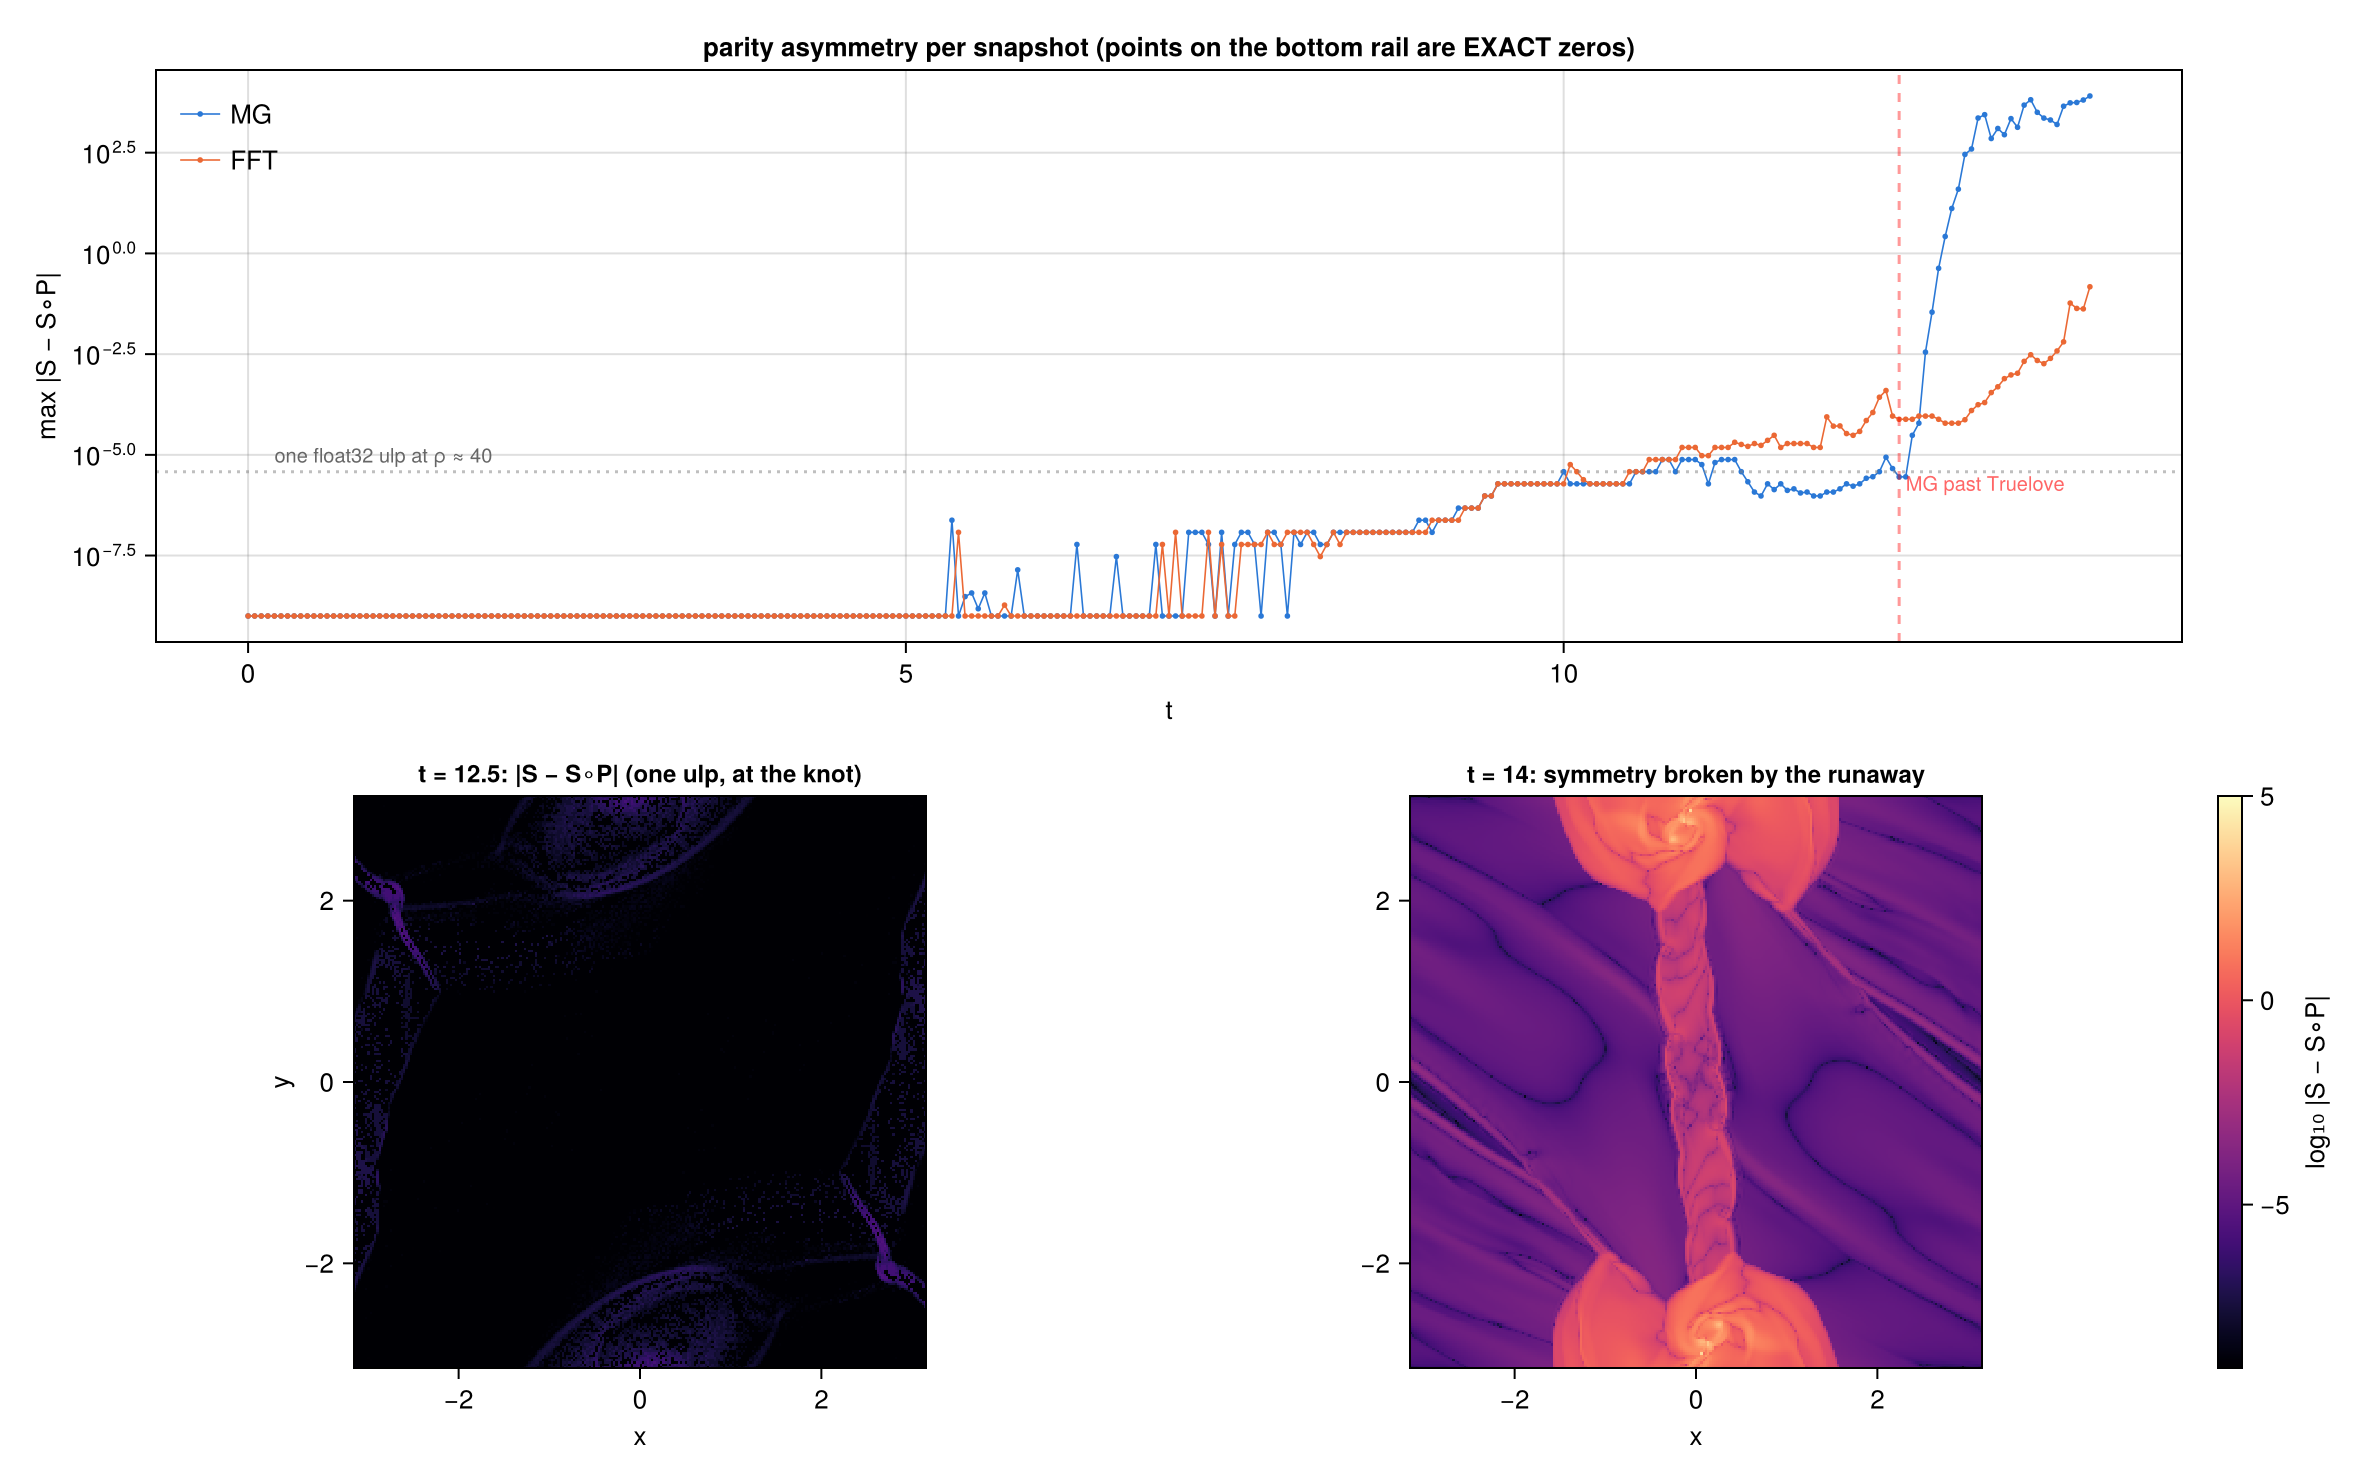
\includegraphics[width=\textwidth]{figures/pi_q21_parity.png}
\caption{The parity measurement. Top: $a(t)$ for MG and FFT --- exact-zero rail,
ulp staircase, explosive break past the Truelove ceiling (red dashed). Bottom:
$|S - S\circ P|$ maps at $t = 12.5$ (one ulp, tracing gradient edges) and $t = 14$
(symmetry broken at the runaway knots).}
\label{fig:parity}
\end{figure}

\end{document}
